This chapter explores into a comprehensive review of theories and literature, including principles, concepts, and ideas applicable in the study. The first part of this chapter includes the discussion of the concept of Calibration theory, Statistical Process Control and Machine learning. The second part of this chapter includes the review of related literature. The Literature Review section synthesizes recent applied research in environmental monitoring. This discussion is organized into targeted subsections evaluating different machine learning methodologies ranging from standalone regression techniques to advanced stacked ensembles and their efficacy in mitigating non-linear cross-sensitivities and hardware drift. Ultimately, this chapter equips the reader with a comprehensive understanding of the physical vulnerabilities inherent in low-cost sensors and the data-driven algorithms necessary to correct them. 

\section{Theories}
\subsection{Calibration theory}
Calibration process involves comparing the results of the device under test to a reference standard and making necessary adjustments to align the device’s readings with the standard \cite{1}. The foundational method used in all calibration is known as Zero and Span Adjustment (Two-point Calibration) which measure two known reference conditions typically a low point near zero and a high point near maximum range. This assumes a linear change in the measured device creating a slope in its error. The Slope for the adjustment is defined as \cite{2} 

\[
M = \left( \frac{A_2 - A_1}{B_2 - B_1} \right)
\]

Where:
\begin{itemize}
	\item $M$ = slope
	\item $A$ = True Value
	\item $B$ = measured value
\end{itemize}

\subsection{Statistical Process Control}
Statistical process control is used for controlling a process using statistical methods to detect the need for calibration \cite{4}. For sensors it is critical to detect when the instrument has drifted. This can be done by applying different methods of statistical process control based on how the drift of the sensor behaves. 

Standard deviation is a statistical method that measures how far numbers in a dataset are spread out from the mean \cite{7}. The equation for standard deviation is defined as

\[
\sigma = \sqrt{\frac{\sum_{i=1}^{n} (a_i - \mu)^2}{n - 1}}
\]

where:
\begin{itemize}
	\item $\sigma$ = Standard deviation
	\item $a$ = place value holder of the entry in the dataset
	\item $\mu$ = mean
	\item $n$ = number of entries in the dataset
\end{itemize}

Cumulative Sum (CUSUM) is a statistical process control method specifically designed to identify subtle, continuous sensor drift over extended deployment periods. Rather than evaluating daily readings in isolation, CUSUM tracks process stability during consistent baseline conditions and accumulates small, deviations that fall below the expected target mean \cite{5}. When the accumulated penalty tally crosses a predefined decision limit typically set at $5\sigma$ of the baseline variance, the system mathematically confirms permanent hardware degradation and triggers a recalibration routine. The CUSUM equation is defined as \cite{6}

\[
S = \max(0, S_{t-1} + (\mu - E) - c)
\]

where:
\begin{itemize}
	\item $S$ = current CUSUM
	\item $S_{t-1}$ = previous CUSUM
	\item $c$ = input
	\item $E$ = error margin
\end{itemize}

A drift is detected when $S > 5\sigma$

\subsection{Machine Learning}
Machine learning is a subfield of artificial intelligence that uses algorithms trained on data sets to create models capable of performing tasks that would otherwise only be possible for humans [8]. A machine learning model receives a dataset D = {X, Y}

\[
X = \begin{bmatrix} 
	x_{11} & x_{12} & \cdots & x_{1m} \\ 
	x_{21} & x_{22} & \cdots & x_{2m} \\ 
	\vdots & \vdots & \ddots & \vdots \\ 
	x_{n1} & x_{n2} & \cdots & x_{nm} 
\end{bmatrix} 
\quad 
Y = \begin{bmatrix} 
	y_1 \\ 
	y_2 \\ 
	\vdots \\ 
	y_n 
\end{bmatrix}
\]

where:
\begin{itemize}
	\item $X$ = input parameters
	\item $Y$ = target parameters
	\item $x$ = input features
	\item $y$ = target
	\item $n$ = number of entries
	\item $m$ = number of features
\end{itemize}

\subsubsection{Random forest} 
Random forest is an ensemble of tree predictors such that each tree depends on the values of a random vector sampled independently and with the same distribution for all trees in the forest \cite{9}. The generalization error for forests converges to a limit as the number of trees in the forest becomes large. The generalization error of a forest of tree classifiers depends on the strength of the individual trees in the forest and the correlation between them.

\begin{enumerate}
	\item \textbf{Hyperparameter} \\
	Random Forest has three standard hyperparameters that are set to configure how the model behaves.
	\begin{itemize}
		\item Trees ($k$) = Refers to the number of trees within the forest, more trees give a more accurate prediction at the cost of more computational power.
		\item Depth ($p$) = Defines how many times each node can split, bigger depth can increase prediction accuracy, but it can also lead to overfitting.
		\item max\_Features ($f$) = Refers to the number of input features that are sampled per node.
	\end{itemize}
	
	\item \textbf{Bootstrapping} \\
	For each tree $n$ number of entries are randomly selected where entries can be repeatedly selected such that $d_k \subseteq D$
	
	where:
	\begin{itemize}
		\item $d$ = randomly selected dataset
		\item $k$ = decision Tree
	\end{itemize}
	
	\item \textbf{Node Splitting} \\
	After each tree is assigned with a randomly selected dataset $d$ a node is created to split the data into two classes, left($L$) and right($R$). To determine which data falls to $L$ \& $R$ a threshold for every element of $d$ is calculated based on the middle value of each element
	
	\[
	s_x = \frac{\max(x) + \min(x)}{2}
	\]
	
	where:
	\begin{itemize}
		\item $s$ = threshold
	\end{itemize}
	
	The values are segregated per features such that every value of the features that are more than the threshold are placed in $R$ while the remaining are assigned to $L$
	
	\[
	R = \{a \in x \mid a > s\}
	\]
	\[
	L = \{a \in x \mid a \le s\}
	\]
	
	After all data for each element have been classed, the MSE of each is Calculated
	
	\[
	MSE_x = \frac{|L_x|}{|x|} \sum_{i \in L_x} (L_x - \overline{L_x})^2 + \frac{|R_x|}{|x|} \sum_{i \in R_x} (R_x - \overline{R_x})^2
	\]
	
	The node is split into $L$ \& $R$ based on the element with the lowest MSE. Node Splitting will keep on recurring until $p$ is reached. At the last node a leaf is calculated to represent the entire tree which is calculated as
	
	\[
	\hat{Y}_N = \sum_{i \in Y} i
	\]
	
	Where:
	\begin{itemize}
		\item $\hat{Y}$ = leaf
		\item $N$ = Node
	\end{itemize}
	
	\item \textbf{Bagging} \\
	During testing the inputs are passed to each tree containing the calculated nodes. Every tree will have a leaf to represent their prediction. To get the final prediction for the model, bagging is calculated as
	
	\[
	Y(x) = \sum_{i=1}^{k} \hat{Y}_i(X)
	\]
	
	where:
	\begin{itemize}
		\item $Y(x)$ = RFR prediction
	\end{itemize}
\end{enumerate}

\subsubsection{Support Vector Regression (SVR)} 
Support Vector Regression is a margin-based regression method that ignores small errors intentionally, it handles nonlinear relationships through kernels and holds up on noisy real-world data where standard regression comes up short \cite{10}.

\begin{enumerate}
	\item \textbf{Standardization} \\
	All inputs are standardized by calculating the mean and the standard deviation of the dataset, calculated as
	
	\[
	\mu_g = \frac{\sum_{i \in D_g} i}{|D_g|}
	\]
	
	\[
	\sigma_g = \sqrt{\frac{\sum_{i \in D_g} (i - \mu_g)^2}{|D_g|}}
	\]
	
	where:
	\begin{itemize}
		\item $g$ = columns in the dataset
	\end{itemize}
	
	Then standardized as
	\[
	Z_g = \frac{D_g - \mu_g}{\sigma_g}
	\]
	
	where:
	\begin{itemize}
		\item $Z$ = standardized input
	\end{itemize}
	
	\item \textbf{Hyperparameters} \\
	
	\textbf{Kernel} ($K(x_i, x_j)$)- The kernel determines how SVR handles patterns in the dataset.
	
	\textbf{Regularization (C)} - $C$ controls how much SVR penalizes errors on points outside the tube. High $C$ means the model takes those errors seriously and fits more tightly. Low $C$ means the model accepts more violations in exchange for a simpler, flatter function.
	
	\textbf{Epsilon ($\varepsilon$)} - Epsilon defines the width of the tolerance margin around the fitted function. A larger $\varepsilon$ means a wider tube.
	
	\textbf{Gamma ($\gamma$)} - $\gamma$ is a special hyperparameter that only exist when the kernel is set to RBF. $\gamma$ defines how far the influence of a single training example reaches, a lower $\gamma$ treats distant points as similar, creating a smoother, more generalized, and linear-like curve.
	
	\item \textbf{Kernel} \\
	The Radial Basis Function (RBF) kernel is used to train nonlinear SVR models which is defined as
	
	\[
	K(x_i, x_j) = e^{-\gamma \|z_i - z_j\|^2}
	\]
	
	where:
	\begin{itemize}
		\item $i, j$ = indices for the dataset
	\end{itemize}
	
	\item \textbf{Weight} \\
	The weight of vectors are calculated as
	
	Where $\alpha_i$ and $\alpha_j^*$ are calculated as
	
	\[
	\max_{\alpha_i, \alpha_i^*} \left[ -\frac{1}{2} \sum_{i, j=1}^{n} (\alpha_i - \alpha_i^*)(\alpha_j - \alpha_j^*) K(x_i, x_j) - \epsilon \sum_{i=1}^{n} (\alpha_i + \alpha_i^*) + \sum_{i=1}^{n} z_i (\alpha_i - \alpha_i^*) \right]
	\]
	
	where:
	\begin{itemize}
		\item $W_i$ = weighted vectors
		\item $z$ = standardized target
	\end{itemize}
	
	With a constraint such that
	\[
	\sum_{i=1}^{n} (\alpha_i - \alpha_i^*) = 0
	\]
	\[
	0 \le \alpha_i, \alpha_i^* \le C
	\]
	\item \textbf{Bias} \\
	A bias of the SVR is calculated as
	
	\[
	b = z_I - \varepsilon - \sum_{i=1}^{n} (\alpha_i - \alpha_j^*) K(x_i, x_I)
	\]
	
	where:
	\begin{itemize}
		\item $b$ = bias
		\item $I$ = chosen index
	\end{itemize}
	
	\item \textbf{Testing} \\
	Using the calculated vectors in the training phase, the predicted values are calculated using the SVR general equation
	
	\[
	f(x) = \sum_{i=1}^{n} (W_i K(x_i, x) + b)
	\]
	
	where:
	\begin{itemize}
		\item $f(x)$ = SVR prediction
	\end{itemize}
\end{enumerate}

\subsubsection{Multiple Linear Regression} 
Multiple regression is an ensemble of linear regressions which is a statistical method used for predictive analysis. It models the relationship between a dependent variable and one or more independent variables by fitting a linear equation to the data. Multiple Linear Regression specifically extends this concept to include two or more independent variables \cite{13}. In MLT beta is describes the linear relationships of the inputs which is defined as

\[
\beta = (w^T w)^{-1} w^T Y
\]

Beta is calculated using a matrix where:
\[
\beta = \begin{bmatrix} 
	\beta_0 \\ 
	\beta_1 \\ 
	\vdots \\ 
	\beta_n 
\end{bmatrix} 
\quad 
w = \begin{bmatrix} 
	1 & x_{11} & x_{12} & \cdots & x_{1m} \\ 
	1 & x_{21} & x_{22} & \cdots & x_{2m} \\ 
	\vdots & \vdots & \vdots & \ddots & \vdots \\ 
	1 & x_{n1} & x_{n2} & \cdots & x_{nm} 
\end{bmatrix}
\]

Using the calculated $\beta$ in the training phase the predicted value is calculated as

\[
g(x) = \beta_0 + \beta_1 x_1 + \beta_2 x_2 + \dots + \beta_n x_m
\]

where:
\begin{itemize}
	\item $g(x)$ = MLR prediction
\end{itemize}

\subsection{Stack Ensemble}
Stack Ensemble is a machine learning technique that builds a new model by combining the predictions of several previously trained models. Stack ensemble takes advantage of mutual complementarity among the base models to improve performance and enhance generalization ability \cite{11}. Stack ensemble works by training multiple models as the basic learner and a second layer of model to serve as the meta learner. The meta learner combines the prediction of the basic learners to create its own prediction as shown in figure 2.1.3.

\begin{figure}[h!]
	\centering
	\includegraphics[width=\textwidth]{stacked.png}
	\caption{Ensemble Stacking}
	\label{fig:ensemble_stacking}
\end{figure}
\subsubsection{Three-way Holdout Split} 
Three-way holdout split is a method for stack ensemble to divide the dataset for training and validation \cite{12}. For a dataset with less than 100,000 entries a split of 50\% basic learner, 25\% meta learner and 25\% validation is a standard. However, for datasets with more than 100,000 entries a split of 98\% basic learner, 1\% meta learner and 1\% validation is used as shown in figure 2.1.3.1.

\begin{figure}[h!]
	\centering
	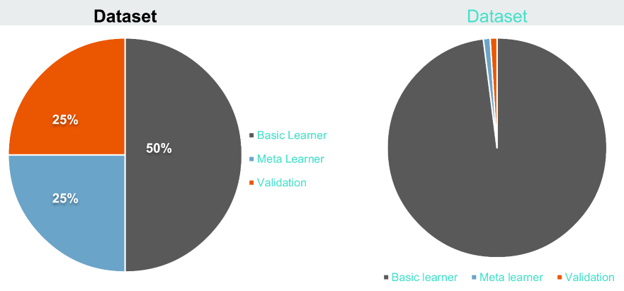
\includegraphics[width=\textwidth]{dataset.png}
	\caption{Three-way holdout split}
	\label{fig:three_way_holdout}
\end{figure}

\subsection{Validation}
Validating the machine learning model performance is a necessary step in machine learning to confirm that the model achieves its intended purpose. Validation is done right after a model is trained and exposed to unseen data \cite{14,17}. Countless validation methods exist for machine learning, however the two methods which are considered as standards for regression models are RMSE and R$^2$.
\begin{enumerate}
	\item \textbf{Root Mean Square Error} \\
	The root mean square error (RMSE) has been used as a standard statistical metric to measure model performance [15]. RMSE measures the average amount of error per prediction, meaning it is in the same unit as the output. RMSE is calculated as
	
	\[
	RMSE = \sqrt{\frac{1}{n} \sum_{i=1}^{n} (y_i - h_i)^2}
	\]
	
	where:
	\begin{itemize}
		\item $h$ = predicted value of the datapoint
	\end{itemize}
	\item \textbf{Coefficient of Determination} \\
	Coefficient of Determination ($R^2$) is used to measure how well a model fits data and how well it can predict. $R^2$ determines how much the variation is in the data. The closer the $R^2$ value is to 1, the better the model fits in the data [16]. The $R^2$ is calculated as
	
	\[
	R^2 = 1 - \frac{\sum_{i=1}^{n} (y_i - h_i)^2}{\sum_{i=1}^{n} (y_i - \bar{y})^2}
	\]
	
	where:
	\begin{itemize}
		\item $\bar{y}$ = mean of target values
	\end{itemize}
\end{enumerate}

\section{Literature Review}
This section investigates the application of machine learning (ML) algorithms for the in-field calibration of low-cost air quality sensors monitoring particulate matter (PM), sulfur dioxide (SO2), nitrogen dioxide (NO2), ozone (O3), and carbon monoxide (CO). While low-cost sensors present a scalable solution to achieve high spatial and temporal resolution in air quality monitoring, their raw measurements often exhibit poor correspondence with professional-grade reference stations. The reliability of these devices is heavily compromised by internal hardware errors and external environmental interferences. Specifically, their performance is notoriously sensitive to non-linear factors such as temperature variations, relative humidity, cross-gas sensitivities, and progressive sensor drift. To bridge this accuracy gap, recent research highlights machine learning as an essential calibration tool. By effectively modelling the complex, non-linear dependencies between environmental confounders and target pollutant signals, ML techniques can dynamically correct sensor data and significantly enhance overall measurement reliability. 

\subsection{Calibration using random forest} %RANDOM FORESTTTTTTTTTTTTTTTTTTTTTTTTTT
The Random Forest (RF) algorithm is widely utilized in air quality monitoring due to its robust ability to reduce model overfitting \cite{concas}. Several studies have demonstrated its efficacy in calibrating low-cost sensors when they are co-located with reference stations. For instance, \cite{Tiago} successfully mitigated cross-sensitivities for CO2 measurements by integrating relative humidity and temperature data, achieving an R2 of 0.93 and an RMSE of 10.93. Their work highlights that in RF training, data diversity is often more critical than dataset size. Similarly, \cite{Ionascu2021} utilized RF to manage cross-sensitivities in Alphasense gas sensors, reporting high correlations for CO (R2 = 0.98) and O3 (R2 = 0.92), although they noted that the sensors struggled at lower pollution detection limits. Supporting these findings, Bush et al. (2022) calibrated multi-pollutant sensors (PM2.5, PM10, and NO2) against reference stations, demonstrating that RF models offer multivariable efficiency, require minimal preprocessing, and are robust to collinearity, yielding strong R2 values ranging from 0.79 to 0.91. 

Conversely, other studies have highlighted the challenges of applying Random Forest in less ideal environmental conditions. While their earlier work was highly successful, a subsequent study by \cite{ionascu2024} demonstrated that RF models struggle when gas concentrations fall near the sensor's lower detection limits. In measuring SO2, NO, and particulate matter (PM) using Alphasense and Plantower sensors, they achieved strong correlations for PM (R2 = 0.94). However, the models yielded significantly lower accuracy for gases like NO (R2 = 0.20) and SO2 (R2 = 0.61) due to the low ambient concentrations in the co-located testing areas. Furthermore, \cite{han} illustrated the critical importance of calibration protocols for RF training. In their measurement of CO, NO2, O3, and SO2, the absence of direct co-location with a reference station resulted in notably poor model performance, yielding low R2 values (e.g., SO2 = 0.012, NO2 = 0.45) and high RMSE readings. Together, these studies suggest that while RF is a powerful calibration tool, its efficacy is highly dependent on sufficient pollution levels and strict co-location procedures. 

Despite these successful implementations, Random Forest models exhibit significant limitations in long-term field deployments. A primary constraint is their inability to extrapolate readings beyond the numerical boundaries of their training data, which can lead to severe inaccuracies during unexpected pollution spikes. Furthermore, RF models struggle with generalizability; their predictive accuracy often degrades when seasonal weather patterns shift outside the parameters observed during their initial training phase. Finally, these models face inherent scalability challenges; because they are heavily reliant on the specific environmental conditions of their co-location site, transferring a trained RF model to a new geographical location typically requires a complete recalibration. 

\subsection{Calibration using other machine learning} %CALIBRATIONNNNNNNNNNNNNNNNNNNNNNNNNNNNNNN ALOT

Various studies have evaluated the efficacy of different machine learning (ML) algorithms in calibrating low-cost environmental sensors. For example, \cite{tastan} assessed the performance of multiple ML models in calibrating a low-cost PMS7003 particulate matter (PM2.5) sensor. By integrating temperature and humidity data from an AHT10 sensor and referencing a Dienmern DM72b monitor, the study demonstrated high predictive accuracy across all tested algorithms. Specifically, tree-based ensemble methods such as AdaBoost (R2 = 0.991, RMSE = 2.541) and Random Forest (R2 = 0.987, RMSE = 2.212) slightly outperformed traditional approaches like Support Vector Machines (R2 = 0.977, RMSE = 2.647). The researchers concluded that integrating meteorological variables significantly improves the accuracy of PM2.5 predictions. 

Similarly, \cite{wang} investigated the calibration of Alphasense sensors for both PM2.5 and nitrogen dioxide (NO2) against Teledyne T640 and Thermo Environmental 42C reference instruments. The authors tested a suite of algorithms, including Random Forest, Support Vector Regression, Artificial Neural Networks, and LightGBM. They found that the Generalized Additive Model exhibited the weakest performance (lowest $R^2$ and highest RMSE). The researchers attributed this lower accuracy to the mobile nature of the deployment and the relatively low pollution levels in the tested areas. 

Expanding on the application of ML across broad geographic areas, \cite{yaqoob} utilized PurpleAir PM2.5 sensors referenced against federal state monitors to evaluate calibration models across multiple states. The researchers compared Random Forest, Linear Regression, Gradient Boosting Regressor, K-Nearest Neighbors, and Neural Networks over a four-year period. Their results indicated that Neural Networks yielded the highest predictive accuracy (R2 = 0.88, RMSE = 1.75 $\mu$g/m$^3$), while traditional Linear Regression and K-Nearest Neighbors demonstrated the weakest performance (both achieving an R2 = 0.83). Notably, the study found that simply adding temperature as a linear correction factor did not significantly improve model performance; instead, non-linear ML models were required to successfully capture the complex interdependencies between environmental features across widespread datasets. 

Recent research has also explored the calibration of agricultural sensors over extended temporal periods. \cite{killeen} investigated nitrous oxide (N2O), pH, and temperature measurements using an LI-8250 Multiplexer and LI-780 Trace Gas Analyzer, referenced against automated gas chambers over a four-year period. The study compared traditional ML models (Random Forest, Linear Regression, Multilayer Perceptron, Support Vector Machine) with tensor-based time-series models (1D-CNN, LSTM). The authors found that LSTM emerged as the most robust and consistent model for both interpolation and multi-year extrapolation tasks (achieving an R2 of 3.30 and RMSE of 3.30 for short-term predictions). Crucially, these non-linear models successfully captured complex agro-environmental interactions without the need for site-specific, process-based parameters. 

However, the long-term stability of these calibration models remains a significant challenge. \cite{barrett} evaluated the calibration of a Winsen MH-Z19C NDIR CO2 sensor against a Picarro G2401 gas analyzer using models such as Random Forest Regression (RFR), Support Vector Regression (SVR), 1D-CNN, and a hybrid CNN-LSTM. Utilizing holdout validation and forward-in-time cross-dataset testing, the study revealed that while calibration accuracy was maintained over a two-month gap between training and testing, performance degraded severely when extrapolated over a 7-month unseen dataset (with all architectures exhibiting weak to negative correlation). Ultimately, the authors found that SVR was the best overall performing model due to its ability to preserve the statistical distribution profile of the reference data while maintaining low error rates. Furthermore, the study noted that training on shorter, contiguous time segments generated lower prediction errors than training on broader time spans, highlighting a major limitation of highly computational, data-heavy models like Neural Networks.

\subsection{Stacked ensemble and hybrid approaches}
%STACKED ENSEMBLEEEEEEEEEEEEEEEEEEEEEEEEEEEEEEEEEEEE
Several studies have explored the efficacy of stacked, ensemble, and hybrid machine learning algorithms across various predictive modeling domains. For instance, \cite{Weimin Wu} investigated the use of a stacked ensemble machine learning model to predict the n-octanol/air partition coefficient (KOA) of Polybrominated Diphenyl Ethers (PBDEs). Their study utilized a super learner framework that integrated Random Forest (RF) and Support Vector Regression (SVR) as base learners in the first layer, with Multiple Linear Regression (MLR) functioning as the meta-learner in the second layer. By leveraging existing chemical databases and density functional theory (DFT) simulations, the researchers demonstrated that this hybrid approach reduced extrapolation errors by 32\% to 48\% compared to individual algorithms. The resulting RF-SVR ensemble model achieved high predictive accuracy, yielding an R2 of 0.981 and a Root Mean Square Error (RMSE) of 0.230. 

Similarly, \cite{tang} applied a hybrid modeling approach to estimate high-resolution PM2.5 mass concentrations over large geographical areas. By combining satellite remote sensing data with observations from meteorological stations, they developed a hybrid model integrating RF and Extreme Gradient Boosting (XGBoost). This RF-XGBoost ensemble yielded an improved RMSE of 7.25 µg/m3, outperforming a standalone RF model, which produced an RMSE of 9.51 µg/m3. This highlights the effectiveness of combining robust tree-based models to capture complex spatial and environmental variables for reliable air quality prediction. 

Recent research has also extended these hybrid methodologies to real-time state-of-charge (SOC) estimation in battery management systems (BMS). \cite{tau} developed a Hybrid Ensemble Dual-State Kalman Filter (HEAD-KF) deployed on an edge computing node (Raspberry Pi 4 Model B). The experimental setup utilized a 20S1P lithium-ion pack with NCA chemistry cells, managed by a BMS with an analog front-end, and evaluated using a 3 kW electronic load cycler. The estimation framework fused XGBoost and RF regressors through non-negative ridge stacking. The output of this ensemble was then refined by a dual-state Kalman Filter, where the process and measurement noise covariances were adaptively auto-tuned in real-time based on residual variance analysis. This methodology perfectly bridges the gap between accuracy and computational cost by combining lightweight, data-driven machine learning with a physics-based, statistical smoother. The approach effectively rejected both high-frequency measurement noise and low-frequency sensor drift, demonstrating the viability of hybrid edge-AI solutions for precise embedded battery management.